\documentclass[xcolor=x11names,compress]{beamer}
%\documentclass[xcolor=x11names,compress, handhouts, aspectratio=169]{beamer}
%% General document
\usepackage{graphicx, subfig}
%% Beamer Layout
\useoutertheme[subsection=false,shadow]{miniframes}
\useinnertheme{default}
\usefonttheme{serif}
\usepackage{palatino}

%%%%%%% Mes Packages %%%%%%%%%%%%%%%%
%\usepackage[french]{babel}
\usepackage[T1]{fontenc}
\usepackage{color}
\usepackage{xcolor}
\usepackage{dsfont} % Pour indicatrice
\usepackage{url}
\usepackage{multirow}
\usepackage[normalem]{ulem}   % For strike out text

% Natbib for clean bibliography
\usepackage[comma,authoryear]{natbib}

%remove the icon
\setbeamertemplate{bibliography item}{}

%remove line breaks
\setbeamertemplate{bibliography entry title}{}
\setbeamertemplate{bibliography entry location}{}
\setbeamertemplate{bibliography entry note}{}

%% ------ MEs couleurs --------
\definecolor{vert}{rgb}{0.1,0.7,0.2}
\definecolor{brique}{rgb}{0.7,0.16,0.16}
\definecolor{gris}{rgb}{0.7, 0.75, 0.71}
\definecolor{twitterblue}{rgb}{0, 0.42, 0.58}
\definecolor{airforceblue}{rgb}{0.36, 0.54, 0.66}
\definecolor{siap}{RGB}{3,133, 200}




%%%%%%%%%%%%%%%%% BEAMER PACKAGE %%%%%%%

\setbeamercolor{itemize item}{fg=siap}
%\setbeamercolor{itemize subitem}{fg=blue}
%\setbeamercolor{itemize subsubitem}{fg=cyan}

\setbeamerfont{title like}{shape=\scshape}
\setbeamerfont{frametitle}{shape=\scshape}

\setbeamercolor*{lower separation line head}{bg=DeepSkyBlue4}
\setbeamercolor*{normal text}{fg=black,bg=white}
\setbeamercolor*{alerted text}{fg=siap}
\setbeamercolor*{example text}{fg=black}
\setbeamercolor*{structure}{fg=black}
\setbeamercolor*{palette tertiary}{fg=black,bg=black!10}
\setbeamercolor*{palette quaternary}{fg=black,bg=black!10}

% Set the header color to SIAP's color
\setbeamercolor*{frametitle}{fg=siap}

%remove navigation symbols
\setbeamertemplate{navigation symbols}{}

\renewcommand{\(}{\begin{columns}}
\renewcommand{\)}{\end{columns}}
\newcommand{\<}[1]{\begin{column}{#1}}
\renewcommand{\>}{\end{column}}

%% Add footer with logo
\setbeamertemplate{footline}{%
  \begin{beamercolorbox}[wd=\paperwidth,ht=2.5ex,dp=1.125ex,%
    leftskip=.3cm,rightskip=.3cm plus1fil]{author in head/foot}
    \includegraphics[height=4ex]{SIAP_logo_Big.png}\hfill
    \insertshortauthor\hfill\insertshorttitle\hfill  \textcolor{siap}{\textit{\insertframenumber}}
  \end{beamercolorbox}%
}

% Path for the graphs
\graphicspath{
{Graphics/}
{c:/Chris/UN-ESCAP/SIAP-E-learning/Resources/OpenScience/}
{c:/Chris/Visualisation/Presentations/Graphics/}
{c:/Chris/Visualisation/Presentations/Graphics/SIAP/}
{c:/Chris/Visualisation/Presentations/Graphics/Lies/}
{c:/Chris/Visualisation/Presentations/Graphics/Maps/}
{c:/Chris/Visualisation/Presentations/Graphics/RGenerated/}
{c:/Chris/Visualisation/Presentations/Graphics/Logos/}
{c:/Gitmain/MLCourse/UNML/Module0/M0_files/figure-html/}
{c:/Chris/UN-ESCAP/MyCourses2022/MLOS2022/Slides/Graphics/}
{c:/Chris/UN-ESCAP/MyCourses2023/RAP/Slides/Graphics/}
{c:/GitMain/RAP/RAP-Course/images/}
{c:/Chris/UN-ESCAP/MyCourses2022/MLOS2022/Slides/Graphics/}
% Path for specific graphs created
 {../R-Codes/JobSatisfaction_files/figure-latex/}
 {../R-Codes/Unused_files/figure-latex/}
 }


\title[\textcolor{siap}{Principles of RAP}]{\textcolor{siap}{Principles of \\ Reproducible Analytical Pipelines \\}
\vspace{0.55cm} \textcolor{brique}{Good practices for \\ Reproducibility}}
\author{Christophe Bontemps}
\institute{\large{\emph{Statistical Institute for Asia and the Pacific} } \\
    \includegraphics[height=10ex]{SIAP_logo_Big.png}}
\date{}


\begin{document}

\begin{frame}
\titlepage
\end{frame}

\section{Reproducibility}

\begin{frame}
\frametitle{Reproducibility}
The term \emph{reproducible} simply means that: \\
\pause
\begin{columns}[t]
 \begin{column}{0.55\textwidth}
    \begin{itemize}[<+->]
    \item[] the \textcolor{siap}{ \textbf{same}} analysis with
    \item[] the \textcolor{siap}{ \textbf{same}} data should lead to
    \item[] the \textcolor{siap}{ \textbf{same}} output (results)
    \end{itemize}
\end{column}
  \begin{column}{0.45\textwidth}
    \begin{center}
    \begin{itemize}
        \only<1-4>{ 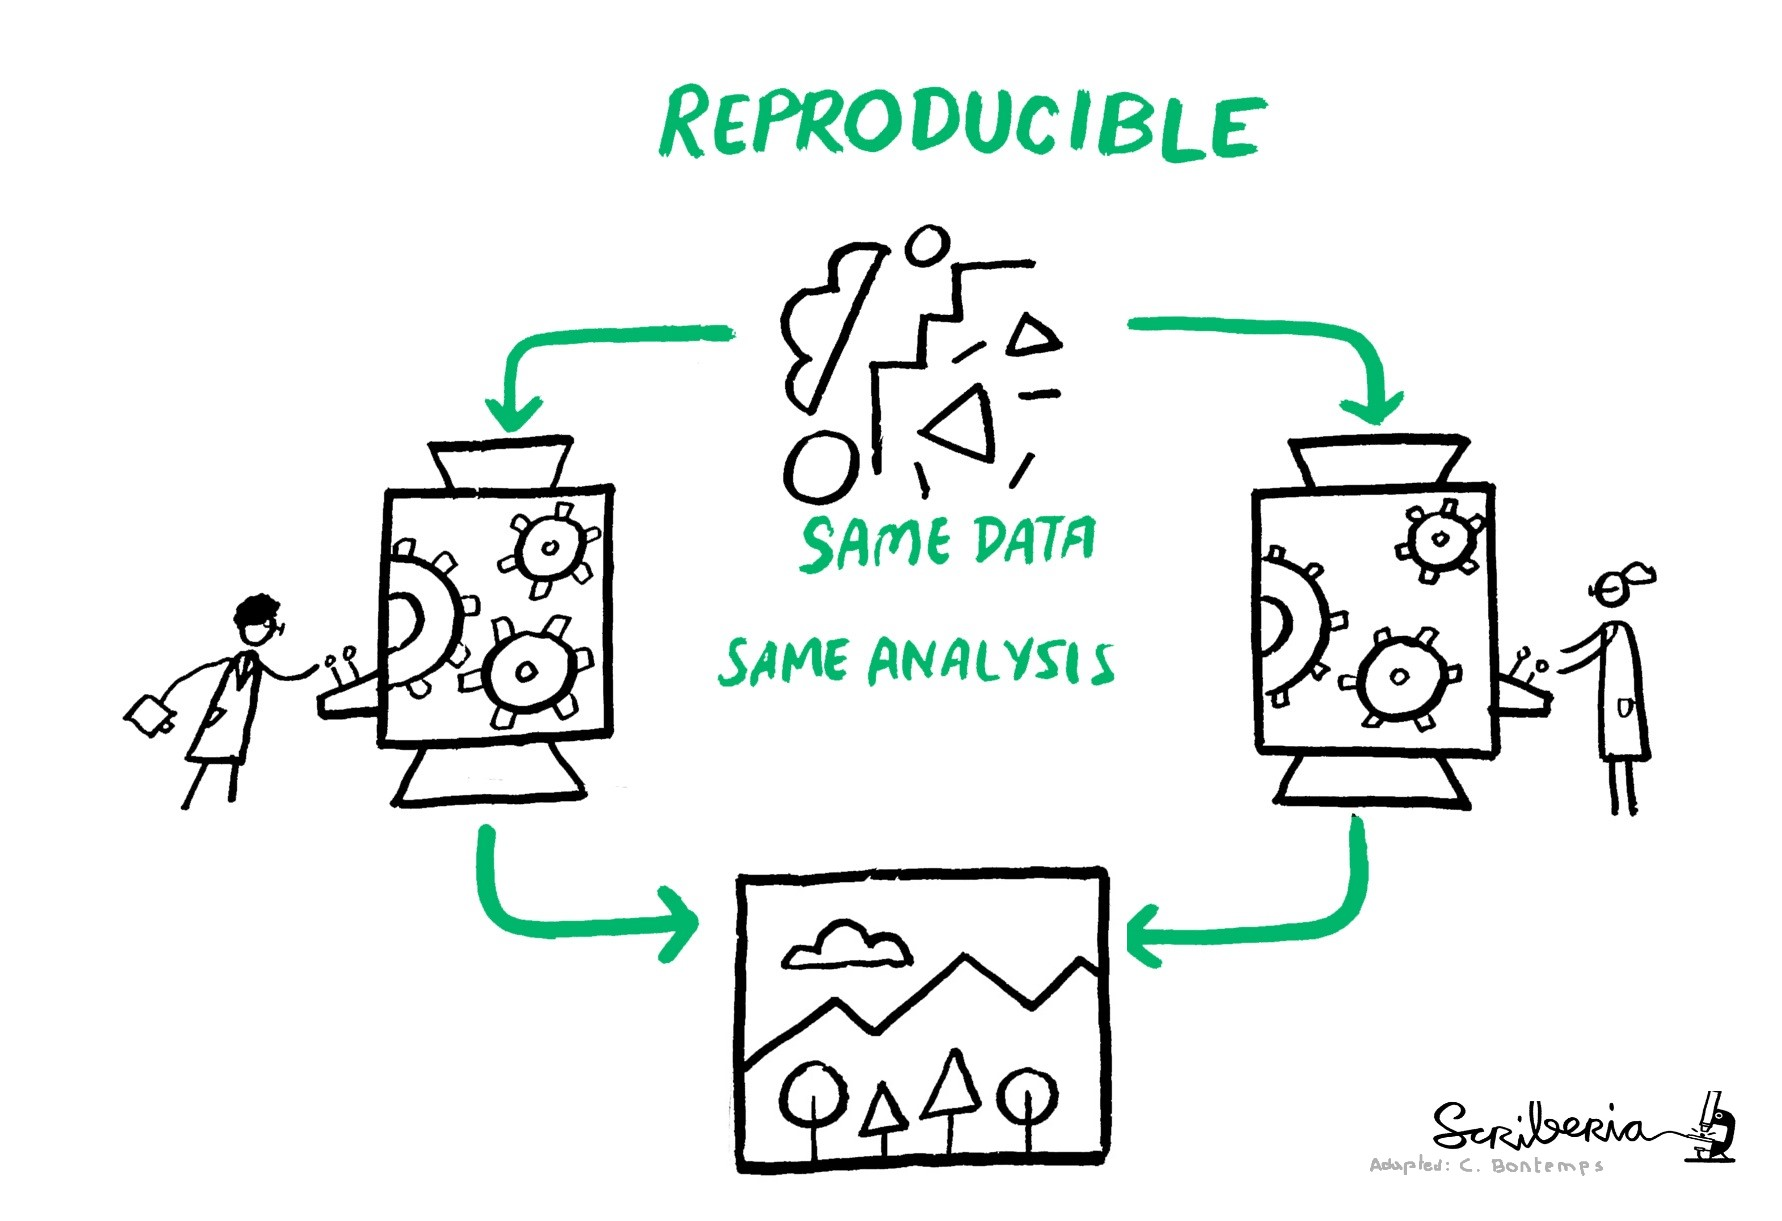
\includegraphics[width=0.95\textwidth]{Reproducible.jpg} \\  }
        \only<1-4>{\hfill  \textcolor{gris}{\tiny{Source: \href{https://the-turing-way.netlify.app/reproducible-research/vcs.html}{The Turing Way project}}}}
    \end{itemize}
    \end{center}
  \end{column}
\end{columns}
\end{frame}


\begin{frame}
\frametitle{Reproducibility}
Related ideas are also interesting: \\
\pause
\begin{columns}[t]
 \begin{column}{0.55\textwidth}
    \begin{itemize}[<+->]
    \item[]\textbf{ Replicable}: The analysis should work with other data
    \item[] \textbf{Robust}:  A different analysis (same data) lead to similar conclusions
    \item[] \textbf{Reusable}: Some elements of the code can be used with other data
    \end{itemize}
\end{column}
  \begin{column}{0.45\textwidth}
    \begin{center}
    \begin{itemize}
        \only<1-4>{ 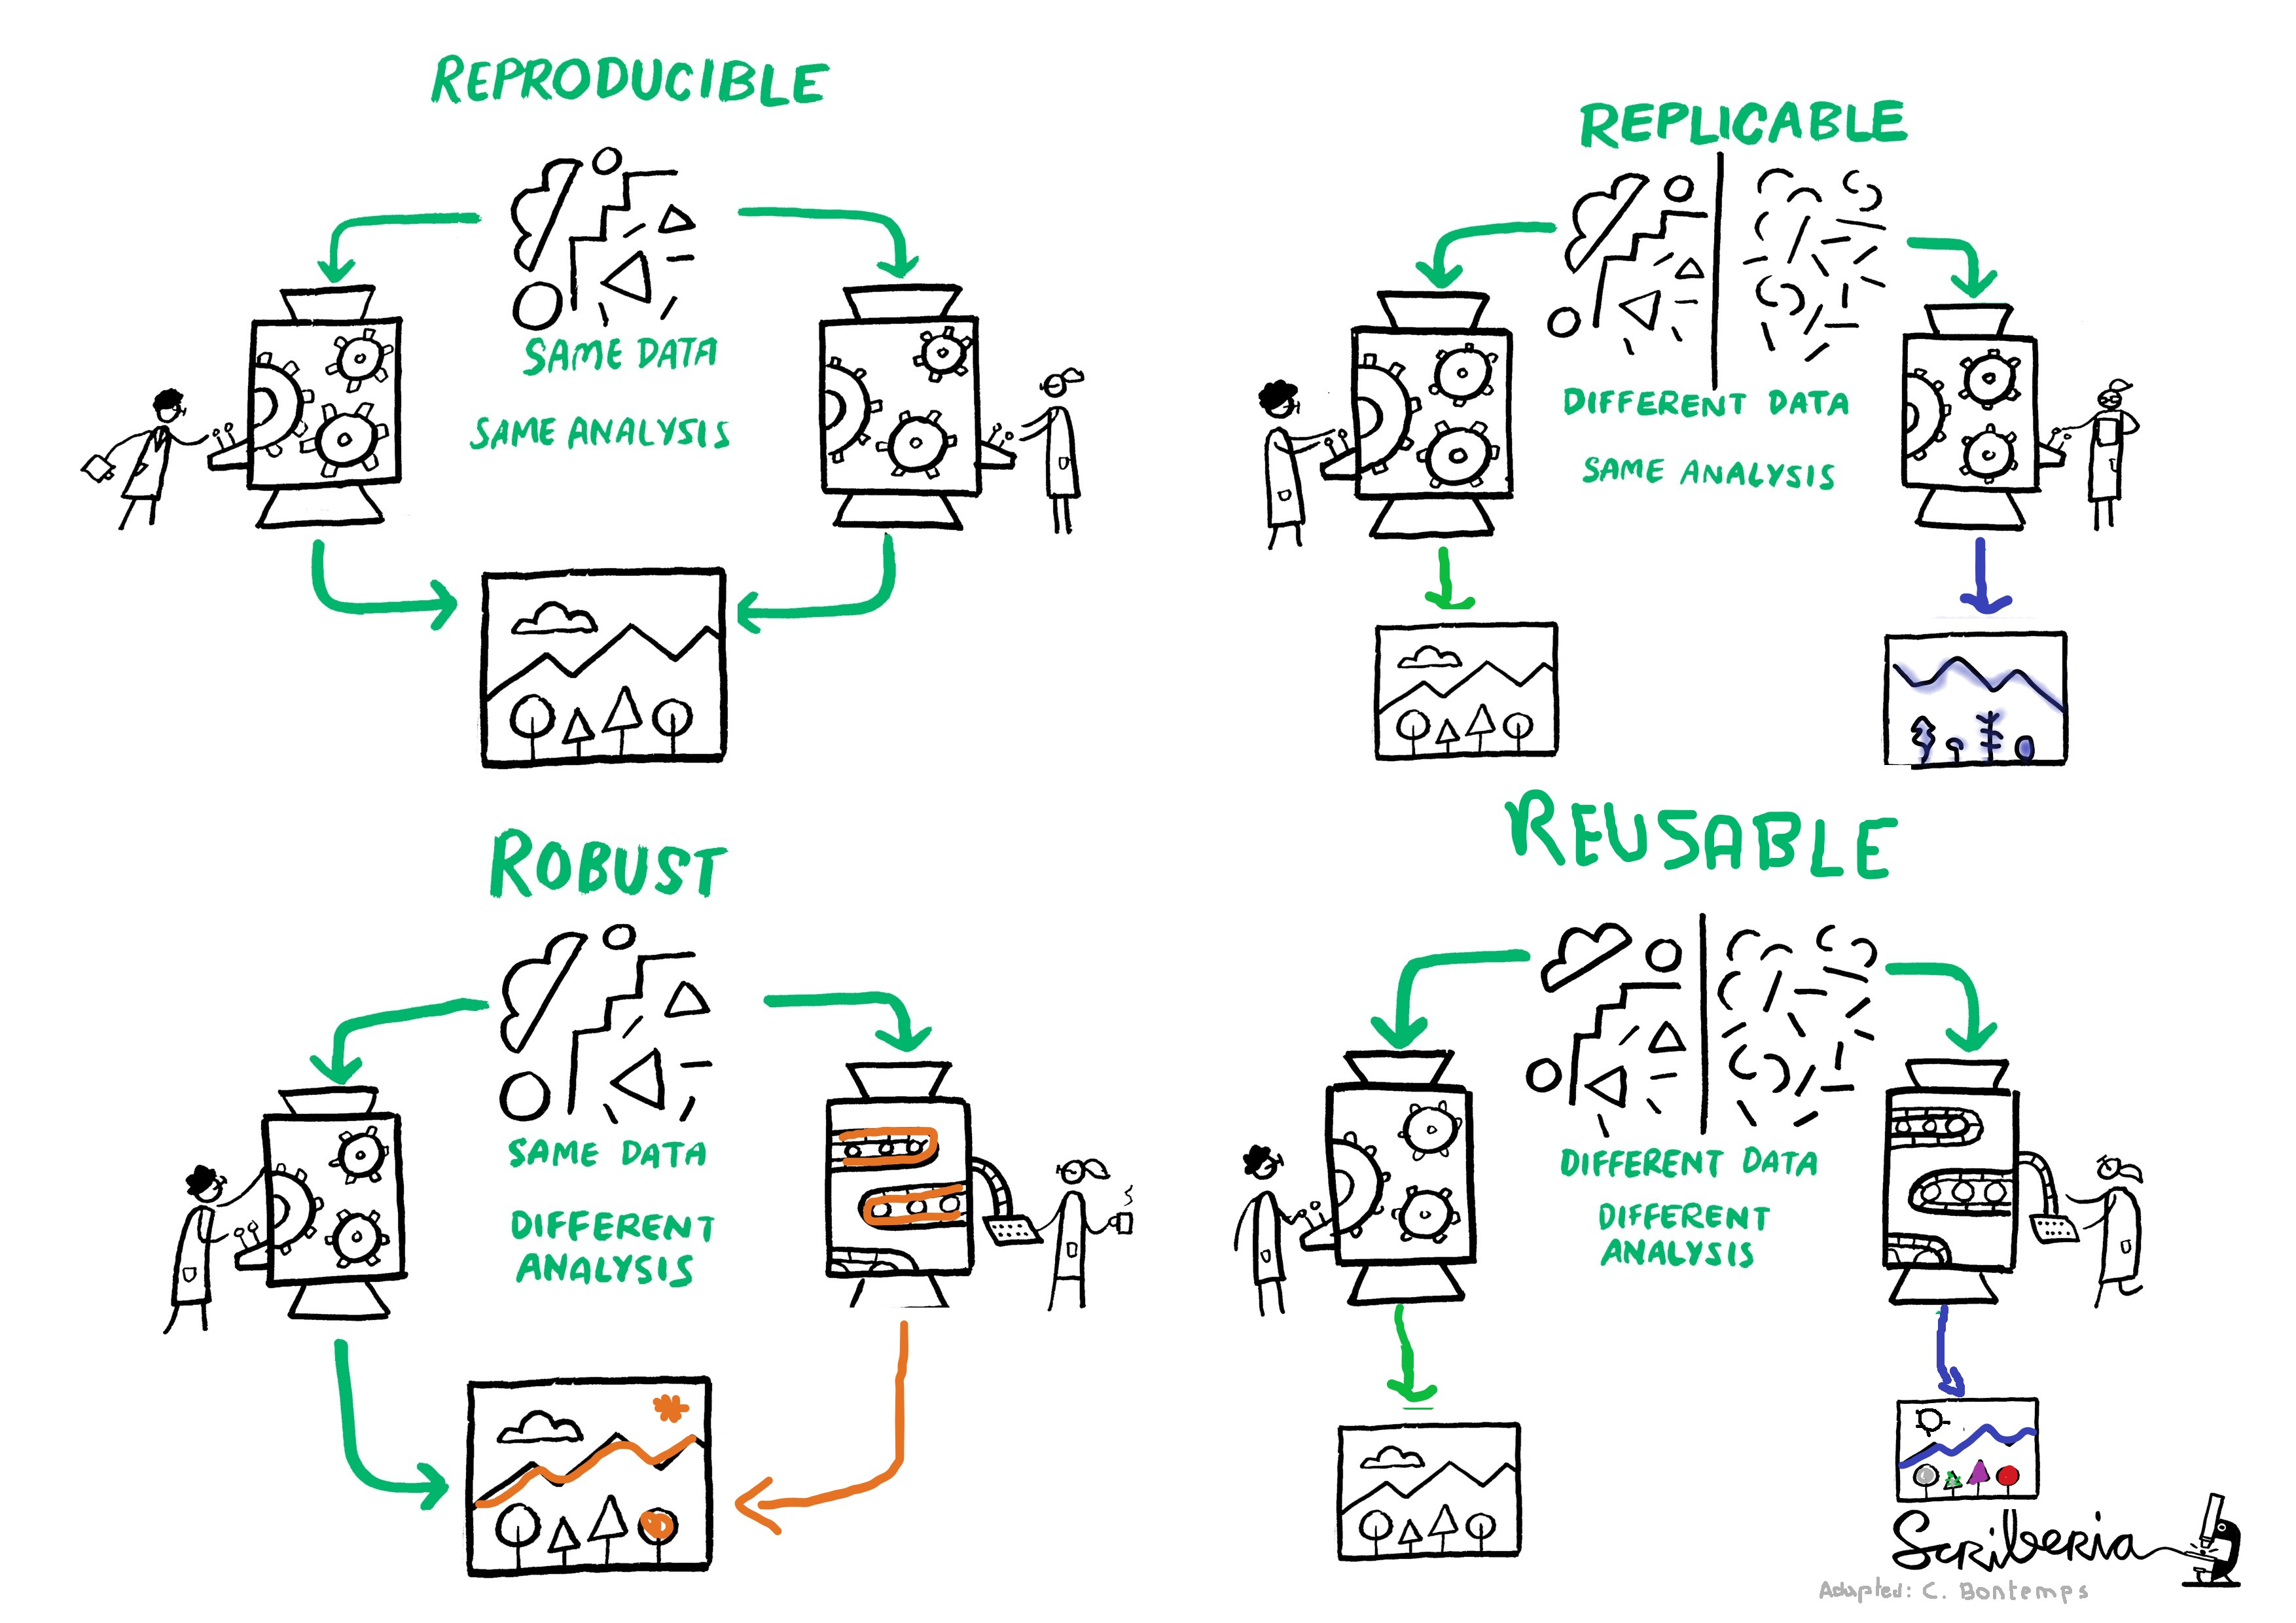
\includegraphics[width=0.95\textwidth]{RRRR.jpg} \\  }
        \only<1-4>{\hfill  \textcolor{gris}{\tiny{\href{https://the-turing-way.netlify.app/reproducible-research/vcs.html}{Adapted from The Turing Way project}}}}
    \end{itemize}
    \end{center}
  \end{column}
\end{columns}
\end{frame}


\begin{frame}[<+->]
   \frametitle{3 main principles:}
    \begin{enumerate}
     \item Organize your work
     \item Code for others (including your future self)
     \item DRY: \textbf{D}o not \textbf{R}epeat \textbf{Y}ourself
      \item[]   \begin{alertblock}{}
            \begin{center}
                  \textit{Apply this in context (colleagues, code, software,...)}
            \end{center}
      \end{alertblock}
    \end{enumerate}
\end{frame}

\section{Organize your work }

\begin{frame}
\frametitle{Organize your work }
\textcolor{siap}{\textbf{Have a clear directory structure}}
 \pause
\begin{columns}[t]
 \begin{column}{0.4\textwidth}

    \begin{itemize}[<+->]
   \item Separate files into data (raw, transformed), programs, results and documentation
   \item Make directories portable (relative path)
    \end{itemize}
\end{column}
  \begin{column}{0.6\textwidth}
    \begin{center}
    \begin{itemize}
         \only<2>{ \includegraphics[width=0.5\textwidth]{WorkingDirectory.png} \\  }
         \only<2>{\hfill \tiny{ \textcolor{gris}{Example of a well-organized directory structure.}}\\ }
         \only<3-4>{\tiny{\textbf{Usual}} \\ }
         \only<3-4>{ \tiny{Mydata <- read.csv("c://document/2024/RAPCourse/Data/TradeData.csv")}  \\ }
         \only<4>{\tiny{ \textbf{Better}}  \\}
         \only<4>{ \tiny{Mydata <- read.csv("Data/TradeData.csv")}  }

    \end{itemize}
    \end{center}
  \end{column}
\end{columns}
\end{frame}


\begin{frame}
\frametitle{Organize your work }
\textcolor{siap}{\textbf{Use naming conventions: } \\ }
For files\\
\begin{columns}[t]
 \begin{column}{0.3\textwidth}
    \begin{itemize}[<+->]
   \item Avoid  lazy names
   \item Meaningful files names
   \item Order of execution
    \end{itemize}
\end{column}
  \begin{column}{0.2\textwidth}
    \begin{itemize}
       \item[]
        \only<1-3>{ \small Usual \\ }
        \only<1-3>{ \small \texttt{prog1.R}\\
                    \texttt{prog2.R}\\
                    \texttt{table.R}\\
                    \texttt{model.R} \\ }
    \end{itemize}
  \end{column}
  \begin{column}{0.5\textwidth}
    \begin{itemize}
        \item[]
        \only<2>{\small Better \\ }
        \only<2>{ \small \texttt{Cleaning\_Data.R}\\
                    \texttt{Stat\_Desc.R}\\
                    \texttt{Statistics\_Trade.R}\\
                    \texttt{Regression\_Trade.R}  }
        \only<3>{\small Even better \\ }
        \only<3>{ \small   \texttt{01\_Cleaning\_data.R}\\
                    \texttt{02\_Stat\_Desc.R}\\
                    \texttt{03\_Statistics\_Trade.R}\\
                    \texttt{03\_Regression\_Trade.R}  }

    \end{itemize}
  \end{column}
\end{columns}
\end{frame}

\begin{frame}
\frametitle{Organize your work }
\textcolor{siap}{\textbf{Use naming conventions:} \\ }
For outputs
\begin{columns}[t]
 \begin{column}{0.3\textwidth}
    \begin{itemize}[<+->]
   \item Avoid numbering
   \item Explicit type of output
    \end{itemize}
\end{column}
  \begin{column}{0.2\textwidth}
    \begin{itemize}
    \item[]
        \only<1-2>{\small Usual \\ }
        \only<1-2>{\small \texttt{Table1.pdf} \\
                    \texttt{Table2.pdf} \\
                    \texttt{Reg1.jpg} \\
                    \texttt{Model.csv} \\ }
    \end{itemize}
  \end{column}
  \begin{column}{0.5\textwidth}
    \begin{itemize}
    \item[]
        \only<2>{\small Better \\ }
        \only<2>{ \small  \texttt{Stat\_Desc\_Table.pdf} \\
                    \texttt{Trade\_Stat\_Table.pdf}\\
                    \texttt{Reg\_Trade\_Graphic.jpg}\\
                    \texttt{Reg\_Trade\_Results.csv} \\ }
    \end{itemize}
  \end{column}
\end{columns}
\end{frame}


\begin{frame}
\frametitle{Organize your work }
\textcolor{siap}{\textbf{Keep track of the workflow:} \\  }
 \begin{columns}[t]
 \begin{column}{0.5\textwidth}
    \begin{itemize}[<+->]
     \item Cut and paste should be avoided
     \item Every step of the process is coded
     \item Manage (and draw) the workflow
   \end{itemize}
  \end{column}
 \begin{column}{0.5\textwidth}
    \begin{itemize}
        \item[]
        \only<1-3>{ \includegraphics[width=1.0\textwidth]{Workflow.png} \\ }
        \only<1-3>{\hfill \tiny{ \textcolor{gris}{Example of a simple workflow.}} }
    \end{itemize}
  \end{column}
\end{columns}
\end{frame}

\begin{frame}
\frametitle{Organize your work }
\textcolor{siap}{\textbf{Use a version control system  (Git/GitHub)}} \\
\vspace{0.5cm}
\begin{center}
 \includegraphics[width=0.7\textwidth]{GitHistory.png}
\end{center}
\end{frame}

\section{Code for others}

\begin{frame}[<+->]
\frametitle{Code for others (including your "\emph{future self}")}
\textcolor{siap}{\textbf{Program with style:}} \\
          \begin{itemize}
             \item Use \emph{literate programming}
             \item[] \begin{center}
                    ``\textit{Let us concentrate rather on explaining to humans \\ what we want the computer to do}'' \\
                    \hfill \textcolor{gris}{ D. Knuth (1984)}
             \end{center}
             \item Use conventions on layout (Comments, indentation,...)  \\
             \href{https://style.tidyverse.org/index.html}{\includegraphics[width=0.5\textwidth]{TidyverseStyle.png}}
         \end{itemize}
\end{frame}

\begin{frame}[<+->]
\frametitle{Code for others }
\textcolor{siap}{\textbf{Program with style:}} \\
  \begin{itemize}
     \item[] Use pipe operator \textbf{\%>\% } ( \emph{tidyverse})
     \item[] \emph{Classic R programming}
     \item[] { \scriptsize   \texttt{nrow(select(filter(TradeData, Export == "Beef"))) }} \\
     \item[]
     \item[] \emph{With pipe operator \%>\% }
     \item[]{ \scriptsize  \texttt{TradeData \%>\% } \\
                            \texttt{  filter(Export=="Beef") \%>\% } \\
                            \texttt{ nrow()} }

 \end{itemize}
\end{frame}

\begin{frame}
\frametitle{Code for others}
\textcolor{siap}{\textbf{Program with style}} \\
\begin{columns}[t]
 \begin{column}{0.3\textwidth}
    \begin{itemize}[<+->]
   \item Avoid ambiguities
   \item Avoid changing units
    \end{itemize}
\end{column}
  \begin{column}{0.7\textwidth}
    \begin{itemize}
    \item[]
        \only<1>{\scriptsize Usual \\ }
        \only<1>{\scriptsize \texttt{sex <- ifelse(gender == "1001", 1, 2)} \\}
        \only<1>{\small Better \\ }
        \only<1>{\scriptsize \texttt{female <- ifelse(gender == "1001",1,0)} \\
                                 \texttt{     male <- ifelse(gender != "1001",1,0)} \\ }
         \only<2-4>{\scriptsize Usual \\ }
        \only<2-4>{\scriptsize \texttt{gdp <- gdp/118.722 } \\
                                \texttt{ } \\ }
        \only<3>{\scriptsize Better \\ }
        \only<3>{\scriptsize \texttt{gdp\_US <- gdp / 118.722}  }
        \only<4>{\scriptsize Even better \\ }
        \only<4>{\scriptsize \texttt{US\_Vanu\_exch\_rate <- 118.722} \\
                                 \texttt{gdp\_US <- gdp / US\_Vanu\_exch\_rate}  }

    \end{itemize}
  \end{column}
\end{columns}
\end{frame}



%%%%%%
\section{DRY}
\begin{frame}
\frametitle{\textbf{D}o not \textbf{R}epeat \textbf{Y}ourself}

\textcolor{siap}{\textbf{Create reusable objects}} \\
\begin{columns}[t]
 \begin{column}{0.2\textwidth}
    \begin{itemize}[<+->]
       \item { \scriptsize Store values}
       \item[]
        \item { \scriptsize Avoid repetitions}
        \item[]
       \item { \scriptsize Use functions}
    \end{itemize}
\end{column}
  \begin{column}{0.8\textwidth}
    \begin{itemize}
    \item[]
        \only<1-2>{\scriptsize Usual \\ }
        \only<1-2>{\scriptsize \texttt{Current\_Data <- subset(Mydata, year  ==2023)} \\}
        \only<2>{\scriptsize Better \\ }
        \only<2>{\scriptsize \texttt{Current\_year <- 2023 \\
                        \texttt{Current\_Data <- subset(Mydata,} \\
                       \hfill \texttt{year == Current\_year)}} \\ }
        \only<3>{\scriptsize Usual \\ }
        \only<3>{\scriptsize \texttt{data <- Mydata[Mydata\$export == "Beef", ]} \\
                 \scriptsize \texttt{plot(data\$Year, data\$Value, } \\
                 \hfill \scriptsize \texttt{ main =  "Export for Beef") \\ }
                 \scriptsize \texttt{  } \\ }
        \only<3>{\scriptsize \texttt{data <- Mydata[Mydata\$export == "Kava", ]} \\
                \scriptsize \texttt{plot(data\$Year, data\$Value, } \\
                 \hfill \scriptsize \texttt{ main =  "Export for Kava") \\ }
                 \texttt{ ... } \\ }
        \only<4>{\scriptsize Better \\ }
        \only<4>{\scriptsize \texttt{ type <- "Beef"} \\
                                \texttt{ } \\
                                \texttt{  Mydata \%>\% } \\
                                \texttt{    filter(exports == type) \%>\%}\\
                                \texttt{    ggplot() + }\\
                                \texttt{    aes(x = Year, y = Value) +}\\
                                \texttt{    geom\_point() + }\\
                                \texttt{    ggtitle(paste("Export for ", type)) }\\
                                \texttt{ } \\ }
         \only<5>{\scriptsize Even better \\ }
         \only<5>{\scriptsize \texttt{Exports\_graphic <- function(type) \{ } \\
                                \texttt{  Mydata \%>\% } \\
                                \texttt{    filter(exports == type) \%>\%}\\
                                \texttt{    ggplot() + }\\
                                \texttt{    aes(x = Year, y = Value) +}\\
                                \texttt{    geom\_point() + }\\
                                \texttt{    ggtitle(paste("Export for ", type)) }\\
                                \texttt{\} }\\
                                \texttt{ } \\
                                \texttt{Exports\_graphic("Beef")} \\
                                \texttt{Exports\_graphic("Kava")   }}

    \end{itemize}
  \end{column}
\end{columns}
\end{frame}

\section{Takeaways}

\begin{frame}
\frametitle{Other principles}
    \begin{itemize}[<+->]
        \item Discuss with colleagues that may use your work
        \item Automatize as much as you can
        \item[$\hookrightarrow$] Reduces your brain's memory burden
        \item There are easy steps everybody can do
        \item[$\hookrightarrow$] Write small programs, one for each task
        \item Use open source program
        \item[$\hookrightarrow$] Easier to share, easier to automatize
        \item[$\hookrightarrow$] Also cost-effective
        \item Test your work regularly:
        \only<11>{\begin{center}
            \emph{``Do what has been said, say what has been done, and \\ check that what has been said has really been done !''}
         \end{center}}
        \only<12>{\begin{center}
            \emph{``\textbf{Code} what has been said, say what has been \textbf{coded}, and \\ check that what has been said has really been \textbf{coded}  !''}
         \end{center}}
    \end{itemize}
\end{frame}



\end{document}



